% =============================% Mon Jan 11 08:35:39 PST 2016% =============================

\subsection*{Direct Form Filters}
We've seen DF1 and DF2. The next step is to transpose them.

\subsection*{Transposition (of a flow graph)}

AKA reverse the flow

(pictures are being drawn here, watch vid5 for more info 1:30ish)



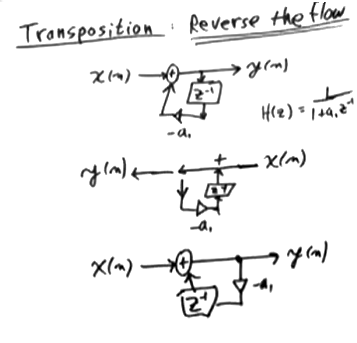
\includegraphics[scale=0.5]{frames/5_a}


\subsection*{DF-1 Biquad}

4:49


$y(n) = b_0x(n) + b_1)x(n - 1)  -
a_1 y(n - 1) - a_2 y(n - 2)
$

*Note process on how he draws it.

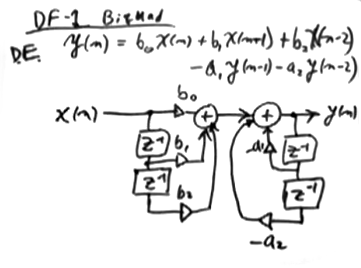
\includegraphics[scale=0.5]{frames/5_b}


\subsection*{DF-2}

around 7:00

Shared delays (more efficient), dangerous intermediate sum that can overflow.

Right: feed forward
left: feed back 
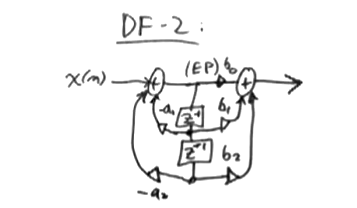
\includegraphics[scale=0.5]{frames/5_c}

\subsection*{Transposed DF-2}
approx 9:00 

\josquote{transposed direct form 2 gets a lot of use}

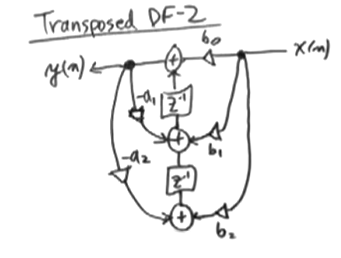
\includegraphics[scale=0.5]{frames/5_d}

\subsection*{FlipLR}
Approx: 11min\\
\josquote{This is the transpose of tapped delay lines... you're summing
into the tapped delay line.}

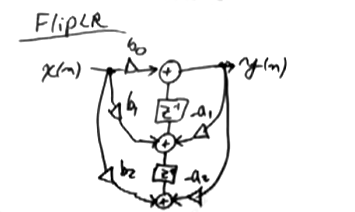
\includegraphics[scale=0.5]{frames/5_e}\\
